\documentclass[conference]{IEEEtran}
\IEEEoverridecommandlockouts
\usepackage{cite}
\usepackage{amsmath,amssymb,amsfonts}
\usepackage{algorithmic}
\usepackage{graphicx}
\usepackage{textcomp}
\usepackage{xcolor}
\usepackage{booktabs}
\usepackage{dblfloatfix}
\usepackage{pdfpages}
\def\BibTeX{{\rm B\kern-.05em{\sc i\kern-.025em b}\kern-.08em
    T\kern-.1667em\lower.7ex\hbox{E}\kern-.125emX}}

\makeatletter
\newcommand{\linebreakand}{%
  \end{@IEEEauthorhalign}
  \hfill\mbox{}\par
  \mbox{}\hfill\begin{@IEEEauthorhalign}
}
\makeatother

\begin{document}

\title{Simple Implementation of Terrain Classification Models via Fully Convolutional Neural Networks\\
{\footnotesize IEEE WinCom 2023 Conference. Istanbul, Turkey}
}

\author{
  \IEEEauthorblockN{1\textsuperscript{st} Assiya Sarinova}
  \IEEEauthorblockA{\textit{Department of Intelligent Systems and Cybersecurity} \\
    \textit{Associate Professor}\\
    \textit{Astana IT University}\\
    Astana, Kazakhstan \\
    ORCID: 0000-0003-4254-376X}
  \and
  \IEEEauthorblockN{2\textsuperscript{nd} Leila Rzayeva}
  \IEEEauthorblockA{\textit{Department of Intelligent Systems and Cybersecurity} \\
    \textit{Assistant Professor}\\
    \textit{Astana It University}\\
    Astana, Kazakhstan \\
    ORCID: 0000-0002-3382-4685}
  \linebreakand
  \IEEEauthorblockN{3\textsuperscript{rd} Noyan Tendikov}
  \IEEEauthorblockA{\textit{Department of Intelligent Systems and Cybersecurity} \\
    \textit{Bachelor Student}\\
    \textit{Astana IT University}\\
    Astana, Kazakhstan \\
    ORCID: 0009-0009-7251-8830}
    \and
  \IEEEauthorblockN{4\textsuperscript{th} Ibraheem Shayea}
  \IEEEauthorblockA{\textit{Electronics and Communication Engineering Department} \\
    \textit{Faculty of Electrical and Electronics Engineering}\\
    \textit{Istanbul Technical University (ITU)}\\
    Istanbul, Turkey \\
    ORCID: 0000-0003-0957-4468}
}

\IEEEoverridecommandlockouts
\IEEEoverridecommandlockouts\IEEEpubid{\makebox[\columnwidth]{ 979-8-3503-2967-4/23/\$31.00~\copyright~2023~IEEE } \hspace{\columnsep}\makebox[\columnwidth]{ }}

\maketitle

\begin{abstract}
This paper introduces a simple implementation of three versions (large, medium, and small) of terrain multi-classification models using Fully Convolutional Neural Networks (FCNNs) for imagery data. The proposed methodology involves labeled and unlabeled data collection from European Space Agency (ESA) WorldCover and Sentinel-2 MultiSpectral Instrument (MSI) on the Google Earth Engine, compressing datasets into Tensorflow records format with 9 diverse terrain types, and handling Google Cloud training computations. There were prepared different dataset portions of 10 megabytes, 200 megabytes, and around a gigabyte files. The experimental results demonstrate the effectiveness of the CNN-based approach, achieving a tolerable 71\% accuracy of the Terrain Classification Model (TCM) and robust classification performance. The simplicity and efficiency of the proposed method make it suitable for real-world applications requiring reliable and fast terrain classification.
\end{abstract}

\begin{IEEEkeywords}
Terrain Classification, Deep Learning, Machine Learning, Aerospace images, Satellite data, Google Cloud Computing
\end{IEEEkeywords}


\section{Introduction}
Geographical data plays a crucial role in our world. In order to ensure its stable and professional transmission, reconnaissance drones or specially designed satellites are widely used. For example, drones, or Unmanned Aerial Vehicles (UAVs), are utilized for specific analytics of limited territorial clusters at nearby distances. In general, their initial mobility makes it possible to obtain information from various perspectives and points of view that is able to improve the completeness of the picture. The current conflict in Ukraine has clearly demonstrated the importance of visual details from scout drones in determining the combat spots of opponents and the navigation of artillery fires on the battlefield \cite{b1}.

Whereas satellites provide a global and qualitative view of the whole Earth’s surface or over large areas in different spectral ranges and time intervals. It adds to the complexity of working with data material but offers valuable insights into separate terrain types and their characteristics, such as land cover mapping, urban planning, agricultural monitoring, or environmental monitoring. The recent waves of wildfires in Russia, Kazakhstan, and Canada have shown the need for early or real-time analytics to prevent incidents, save lives, and optimize the performance of various preservation services. Thus, satellite terrain image classification is an efficient automated approach to extracting valuable insights from its large volumes of data. It is a multiphase workflow that requires parsing data from Geographic Information Systems (GISs), grouping pixels, data mining, algorithmization, etc.

\section{Overview}
GIS experts distinguish 3 primary categories of classification: automated, manual, and hybrid (a combination of automated with manual) \cite{b2}. As shown in the Figure 1, automated types are implemented systematically via supervised (labeled data) and unsupervised (unlabeled data) methods. The research of Al-Ahmadi and Hames \cite{b3} was presented about ISODATA unsupervised classification with repeatedly dynamic partitioning and merging of clusters of images for a predefined amount of iterations. It is a more complicated approach than Support Vector Machine (SVM), Random Forest (RF), Decision Trees (DT), and K-Means techniques. They are commonly used for fast executions. For example, methods or models in the RF category can present up to 89\% accuracy for tasks such as identifying agricultural cropland in South Asia based on an open Google Earth dataset \cite{b4}. On top of that, Duro et al. \cite{b5} compared pixel-based and object-based datasets of SPOT-5 HRG and found that trained RF and SVM machine learning models are able to get the same results in the case of accuracy of agricultural landscape recognition, which is over 90\% for both cases.

\begin{figure}[htbp]
\centering
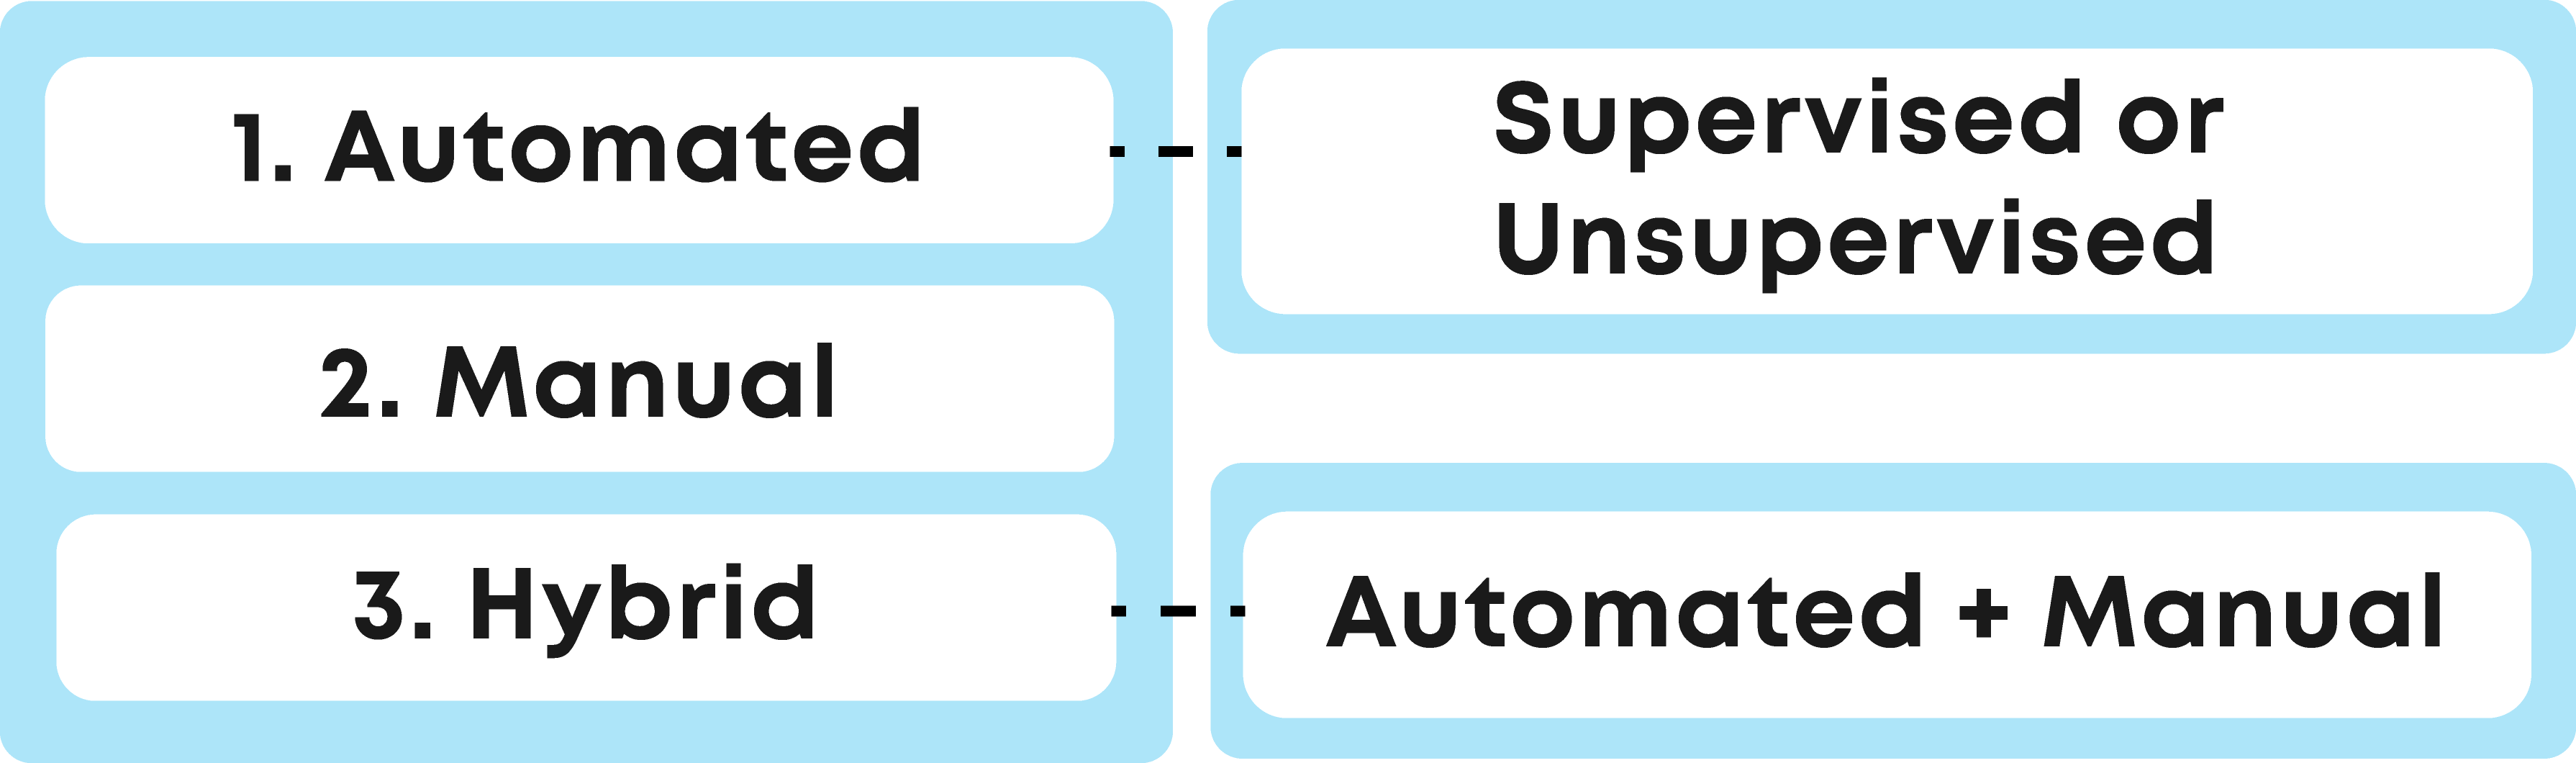
\includegraphics[width=1\linewidth]{fig1.png}
\caption{Satellite terrain image classification methods.}
\label{fig}
\end{figure}

However, machine learning models are limited to the initial augmented data and cannot be applied globally. According to the research of Regan et al.\cite{b6}, deep learning architectures based on CNNs connections are able to identify different visual figures from large datasets. It is shown that some parameters can be combined in multiple layers in order to make more complicated models, such as VGGNet, ResNet50, SegNet, U-Net, PSPNet, and others. For example, Jeppesen et al. \cite{b7} demonstrated that the implementation of RS-Net (a modified version of U-Net) for the Landsat 8 dataset could detect cloud patterns in less than 34 seconds per image product. In addition, in the research of Zhang et al. \cite{b8}, it was shown that a patch-based CNN model that is trained on the same Landsat dataset is able to get an overall accuracy of 97\% in the task of only detecting rice plantations near rivers in the China region. This brought us a final, solid understanding that CNN-type models are absolutely required in the project.

\section{Methodology}

\subsection{Dataset Evaluation}\label{AA}

As a means of developing testing and training data collections, two large datasets have been selected from European satellites: Sentinel-2 MSI and ESA WorldCover. They are available completely free to download from the Google Earth Engine servers or upon request from their API \cite{b9}. Sentinel-2 consists of a constellation of satellites that constantly provide high-resolution optical imagery of the Earth's surface within 5 to 10 days \cite{b10}. This dataset is frequently used by governmental or private organizations to plan urban and agricultural monitoring. Although MSI means that it as well consists of multiple spectral ranges, the train data is implemented using only RGB human-visible planes. On the other hand, ESA WorldCover is based on Sentinel-2 and Sentinel-1 data with 10 meters of resolution per pixel. Its products have 11 terrain cover classifications, including "Tree cover", "Grass land", "Built-up", etc. 

Firstly, in this project was practiced the merging of these 2 datasets. ESA WorldCover was used for primary labeling of data regions, but types of classification were limited to 9 amounts: "water", "trees", "grass", "flooded Vegetation,", "croups, "shrub and scrub", "built-up Areas,", "bare Ground,", "snow and Ice.". However, ESA WorldCover consists only of land cover data, so missed values for ocean regions were filled with the "water" class. Secondly, there are applied Google Cloud Services, which optimize work with data and allow it to be stored or processed in a dedicated bucket. Referring to the Figure 2, Google Cloud Dataflow with Apache Beam constructs a pipeline for dataset creation by creating shapes of regions in Google Earth Engine and getting sample point examples.

\begin{figure}[htbp]
\centering
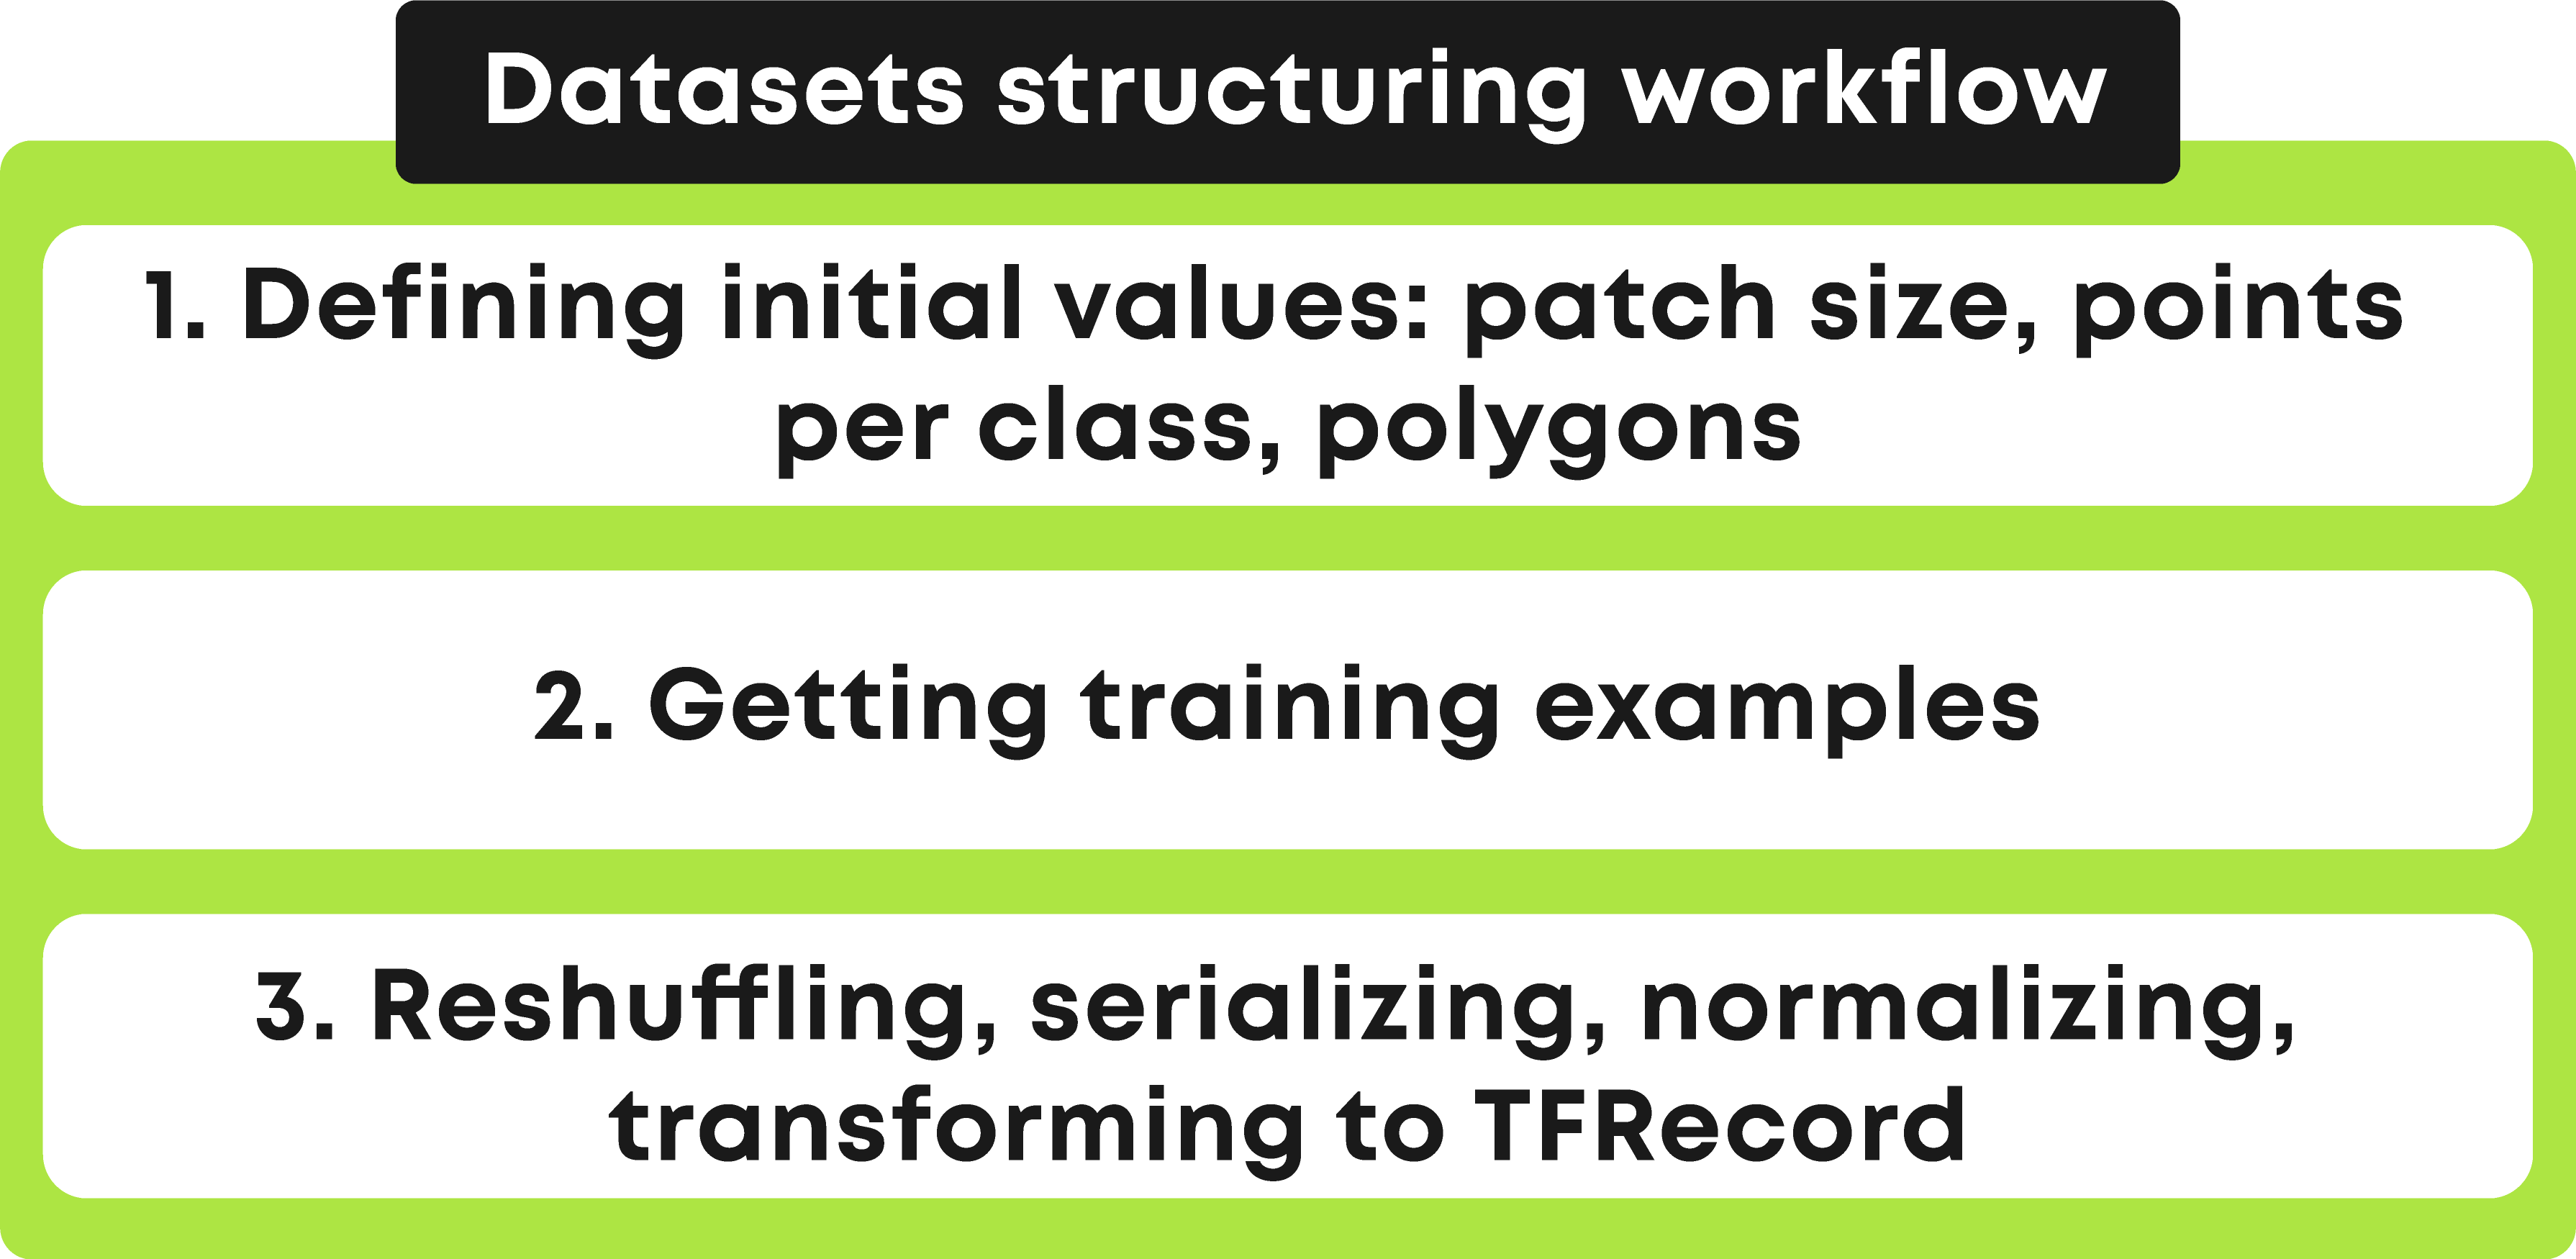
\includegraphics[width=1\linewidth]{fig2.png}
\caption{Workflow of datasets structuring.}
\label{fig}
\end{figure}

There are only a few significant continents or regions of the world represented in this sample, including Europe, Asia, Africa, Australia, North America, and South America, as illustrated in the Figure 3. Thirdly, Apache Beam compresses numpy arrays into a single TensorFlow record. Therefore, for the project, three different datasets were prepared: large (over 1 gigabyte), medium (around 200 megabytes), and small (around 10 megabytes). The final size depends on sampling parameters such as region size or amounts, types of categories, stratification, normalization, and so on.

\begin{figure}[htbp]
\centering
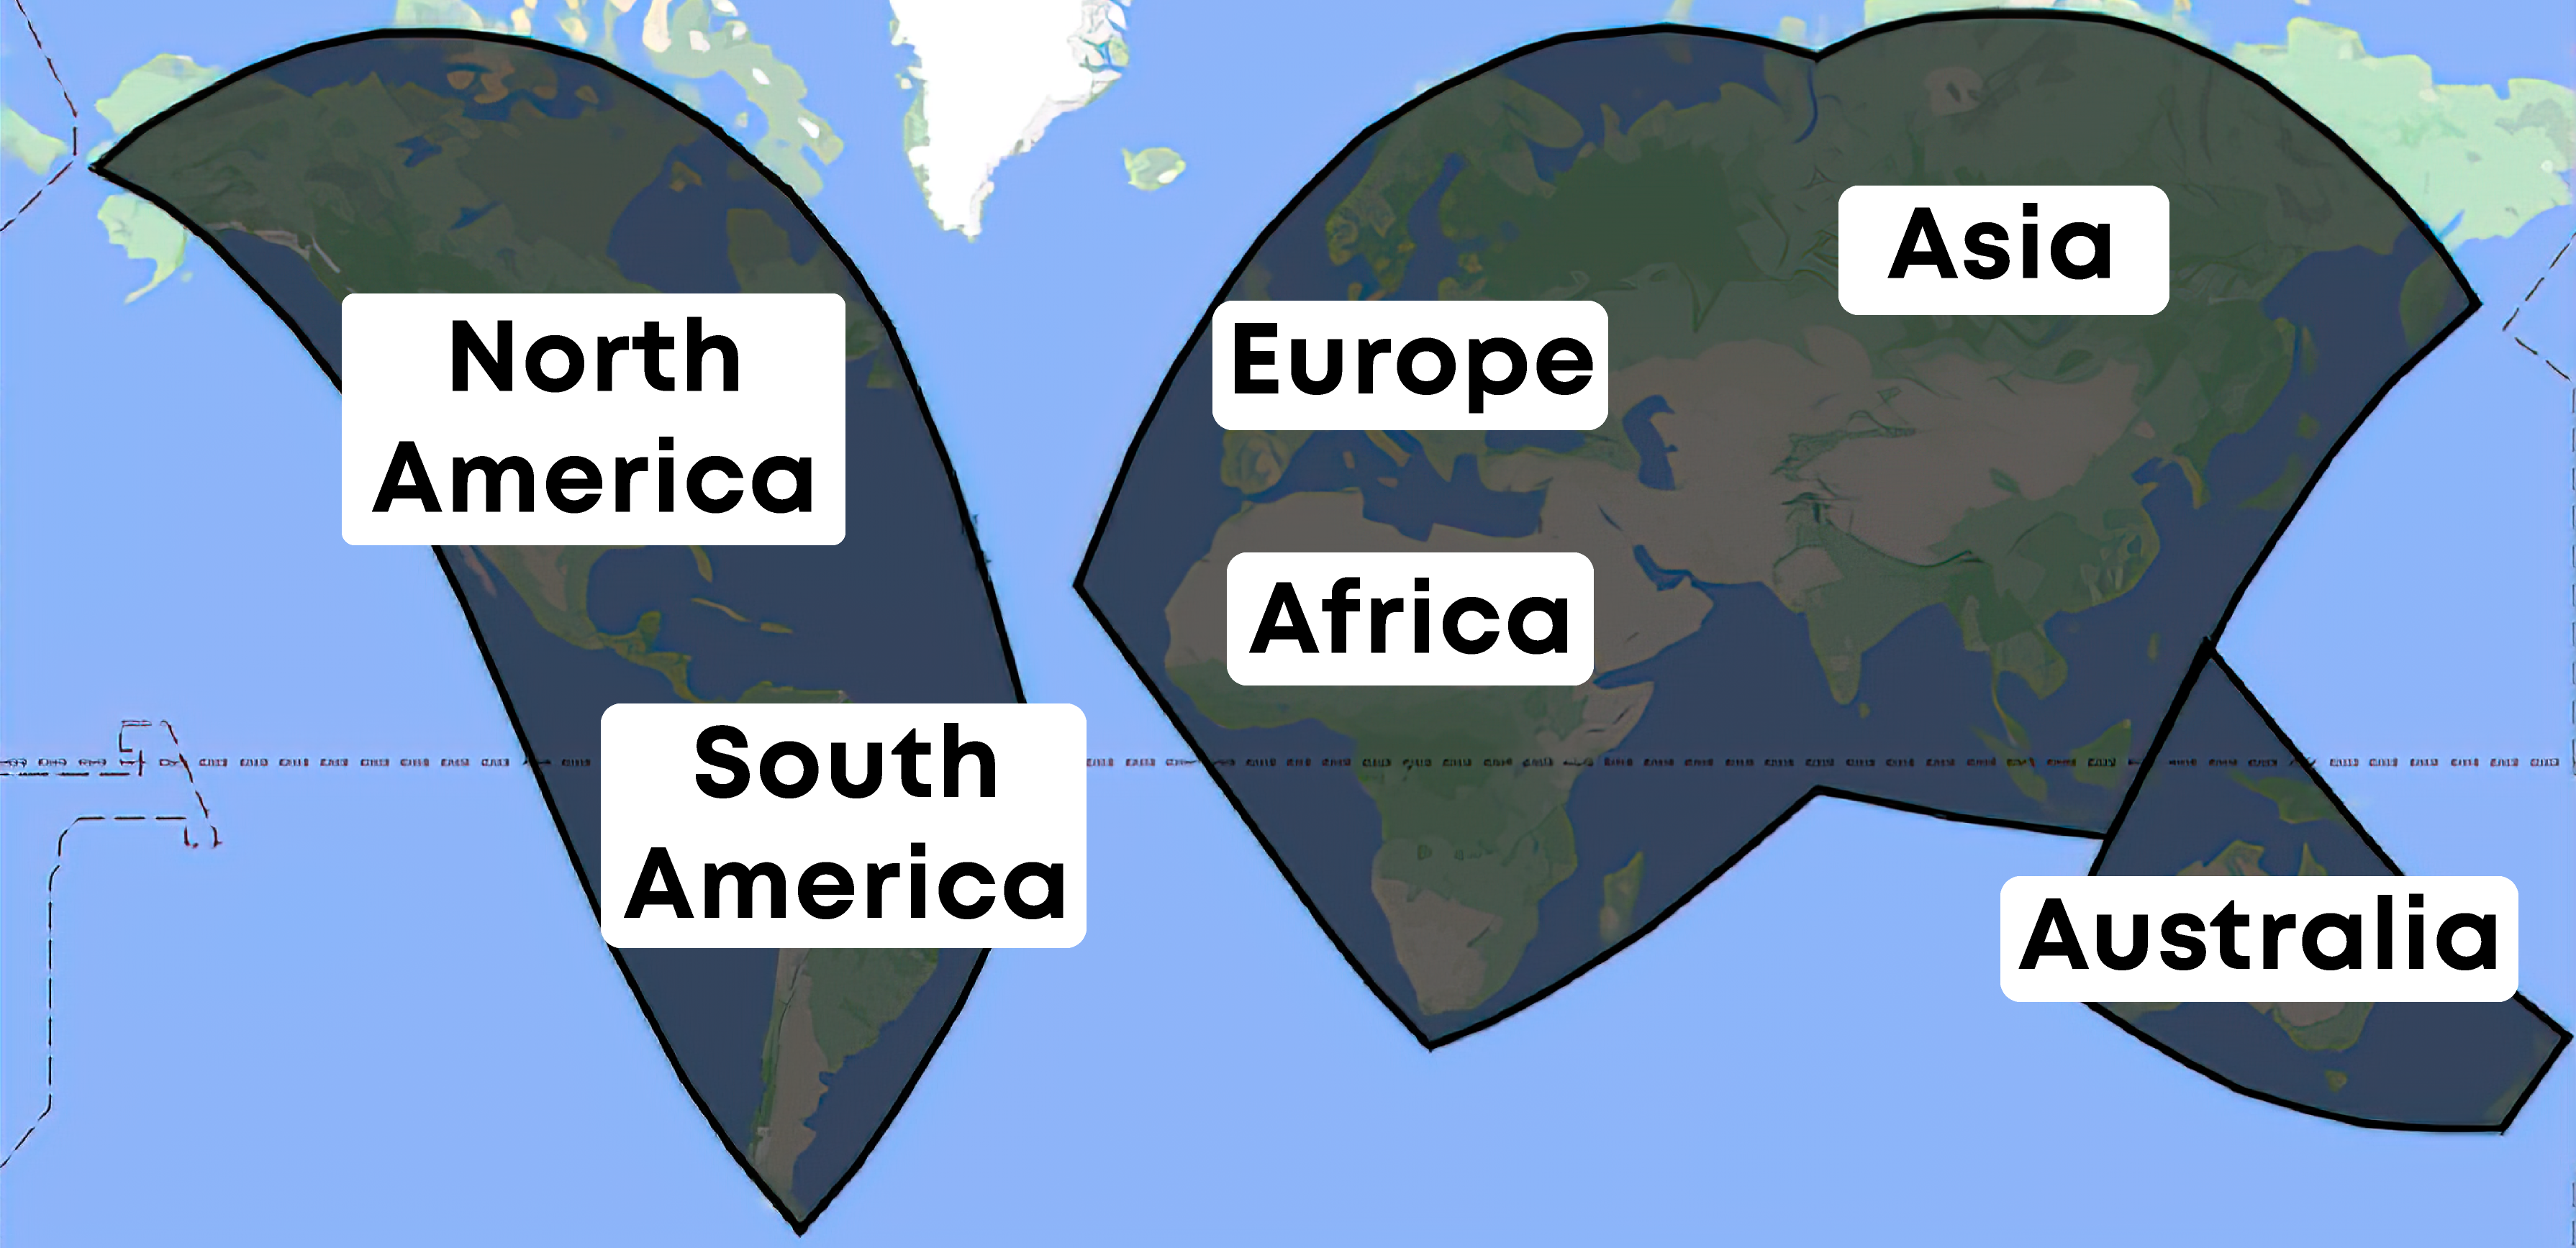
\includegraphics[width=1\linewidth]{fig3.png}
\caption{Example of polygon areas for training data that cover most land territories.}
\label{fig}
\end{figure}

\subsection{Model Architecture and Training}\label{AA}

In this case, the TensorFlow Keras Python library was utilized to design and implement the FCNN model. It contains various prebuilt patterns for neural networks and deep learning.

\begin{figure*}[htbp]
\centering
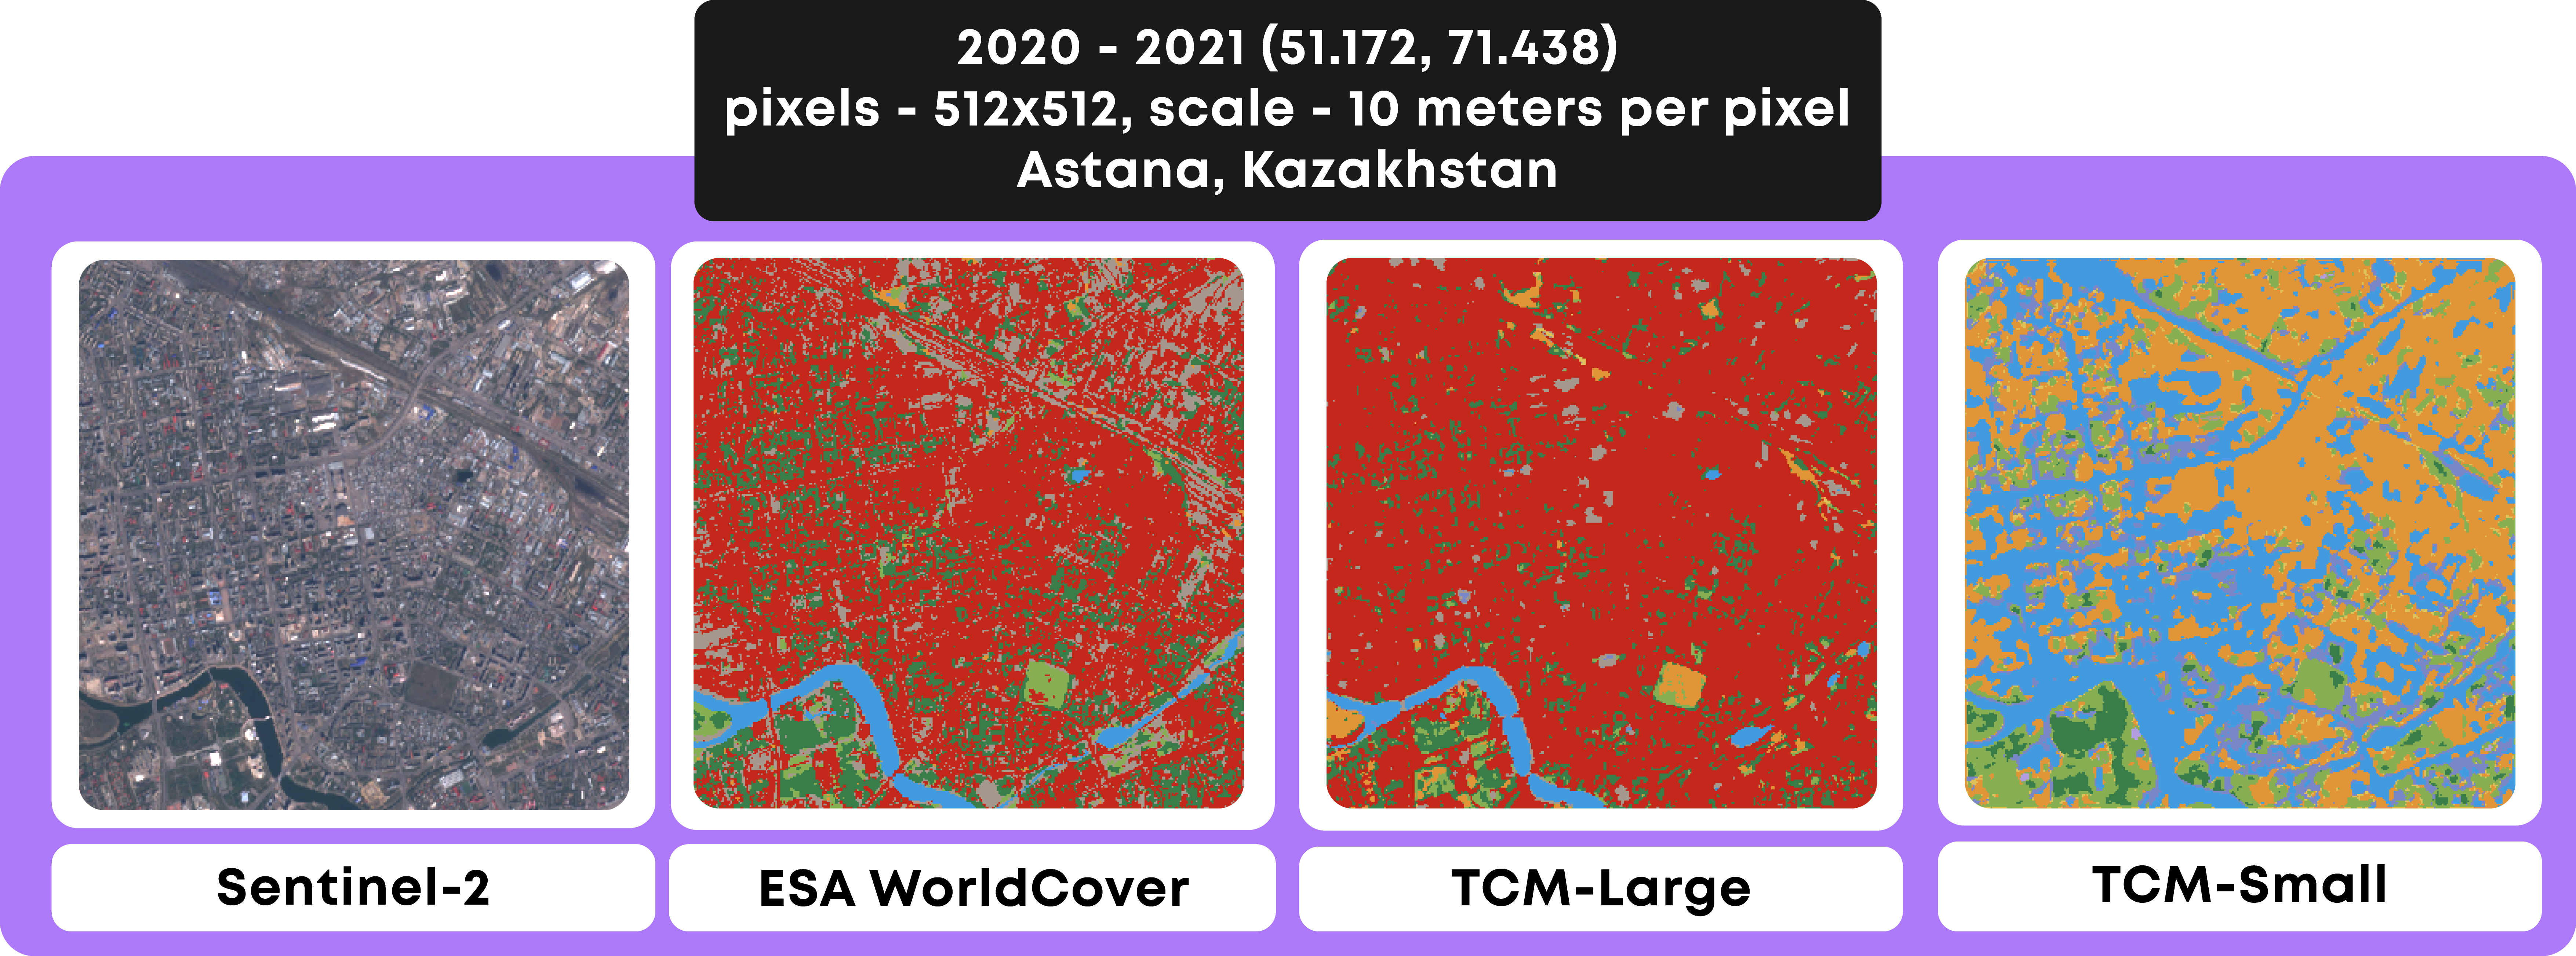
\includegraphics[width=1\linewidth]{fig5.png}
\caption{Visual predictions comparison of models.}
\label{fig}
\end{figure*}

So, Keras greatly simplifies the implementation of the project by combining diverse structures and functions. The Figure 5 demonstrates that the structure of the final model contains an input layer, a normalization or preprocessing layer, convolutional with deconvolutional layers, and an output layer. All the previously listed layers are fully connected. It means that they connect all the neurons or parameters from the previous layer to another subsequent layer, facilitating complex relationships. 

Firstly, the input layer receives a dense tensor of information formed from patch size (vertical and horizontal) and number of bands (Sentinel-2 MSI has only 13 of them). This layer does not transform data into any formats. Secondly, the preprocessing layer is an additional layer that standardizes or normalizes the inputs of the initial training dataset in order to improve stability and prevent the dominance of several features. Thirdly, convolutional layers are responsible for capturing local features that detect imagery patterns. They classify pixels step by step around any kernel with some padding around it. Finally, the output layer is based on the idea of activation functions. This function is able to output specific values when a certain neuron threshold is exceeded. The values are given in the format of the multi-class classification distribution of labels.

\begin{figure}[htbp]
\centering
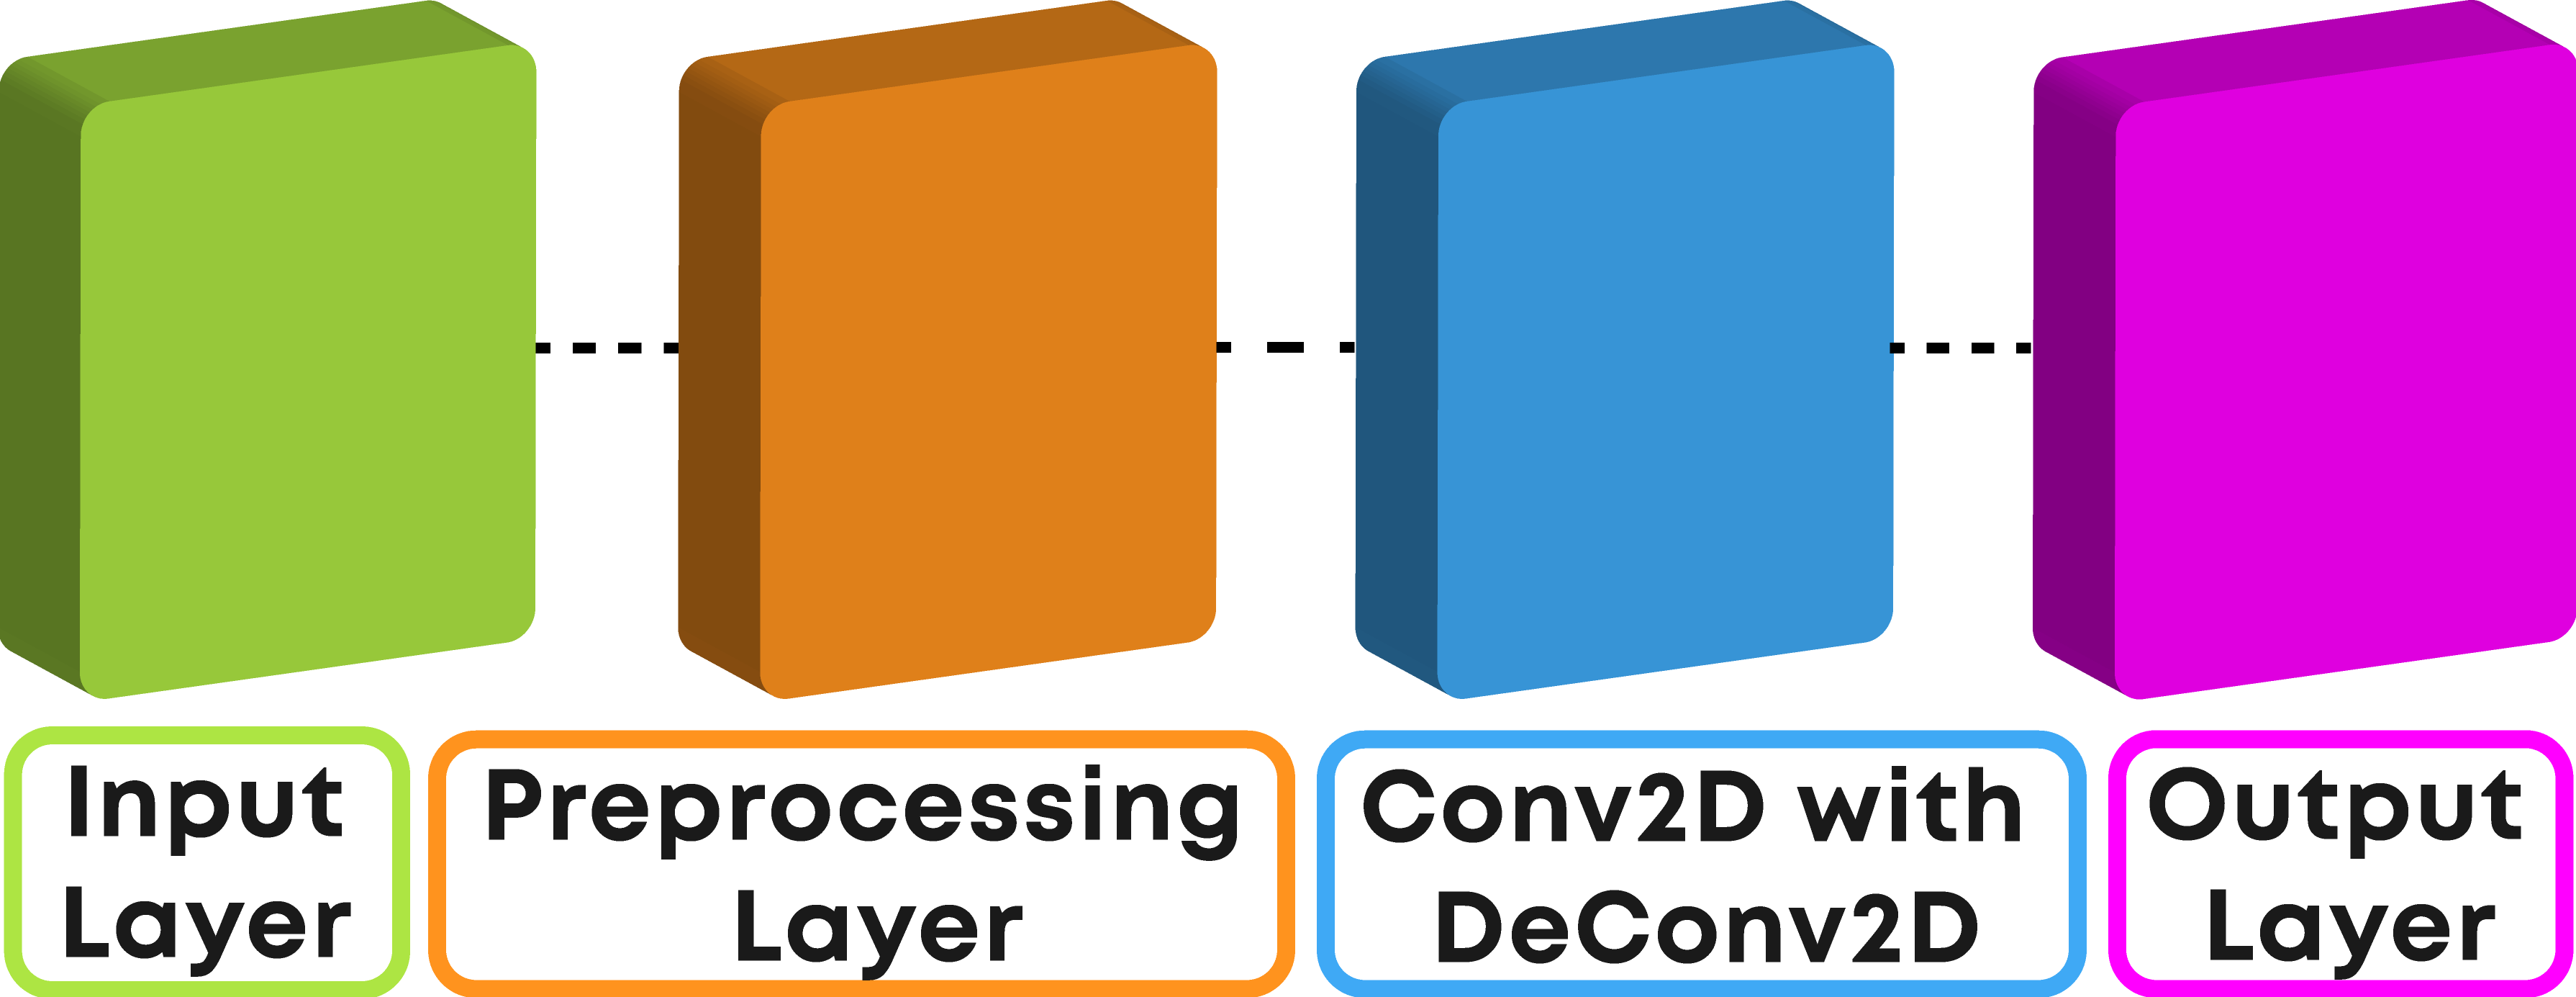
\includegraphics[width=1\linewidth]{fig4.png}
\caption{FCNN-based terrain classification model architecture.}
\label{fig}
\end{figure}

The models were trained on the basis of Google Vertex AI through interaction with the json web token in Google Colab. Google Vertex AI is known as the leading platform for automating machine learning and model deployment, which greatly simplifies the scaling process \cite{b11}. For this project, a separate dedicated Auto-ML custom container from Google was used with the following characteristics: Container - europe-docker.pkg.dev, CPU - e2-standard-8. During this training process, the Adam optimization technique repeatedly updates the parameters of the model. It is practiced for the minimization of a defined loss function, or cross-entropy loss. As a result, there were trained three terrain classification models (TCM): TCM-Large, TCM-Medium, and TCM-Small.

\subsection{Evaluation metrics}
As a way of checking the results of the models, various visual and mathematical indicators are used. In this case, only the main ones were applied that are applied in the evaluation of a classification or prediction model, namely precision, recall, F1-score, and accuracy. Firstly, precision and recall are basic values that show ratios between positive and negative predictions. Secondly, the F1-score shows balance between precision and recall using their harmonic mean. Lastly, accuracy measures overall correctness by dividing true positives and true negatives by total instances.

\begin{equation}
Precision = \frac{TP}{TP+FP} \\[5pt]
\end{equation}

\begin{equation}
Recall = \frac{TP}{TP+FN} \\[5pt]
\end{equation}

\begin{equation}
F1 = \frac{2*Precision*Recall}{Precision+Recall} \\[5pt]
\end{equation}

\begin{equation}
Accuracy = \frac{TP+TN}{TP+TN+FP+FN}
\end{equation}

\section{Results and Discussions}

The models were trained, which took a total of 50 minutes for unique epochs, with TCM-Large taking up the majority of that time. However, according to the results of training with a different number of epochs, and the size of the training data, the trend is clearly visible that TCM-Large shows the best results. For visual analysis in the Figure 4, here is an urbanized region in Astana city of Kazakhstan that has a combination of many details of vegetation, water, and buildings. It displays agile and more obvious distributions of areas with an accurate classification by region and type. Furthermore, it demonstrated "relatively" acceptable indicators of qualities: average precision - 0.67, recall - 0.71, F1-score - 0.65, accuracy - 0.71. It can be seen from the sampling results in the Table 1.

\begin{table}[htbp]
\centering
\caption{Precision, accuracy, recall, F1-score of TCM models}
\label{tab}
\begin{tabular}{l|c|c|c}
\toprule
\textbf{Models} & \textbf{Precision} & \textbf{Recall} & \textbf{F1-Score}\\
\midrule
TCM-Large (macro avg) & 0.38 & 0.32 & 0.32\\
TCM-Large (weighted avg) & 0.67 & 0.71 & 0.65\\
TCM-Small (macro avg) & 0.23 & 0.44 & 0.06\\
TCM-Small (weighted avg) & 0.78 & 0.06 & 0.05\\
\bottomrule
TCM-Large (accuracy) & & & \textbf{0.71}\\
TCM-Small (accuracy) & & & \textbf{0.06}\\
\bottomrule
\end{tabular}
\end{table}

On the other hand, the experimental model TCM-Small showed substandard results in the form of accuracy - 0.06 for obvious reasons. Because of the special allocation of the smallest possible dataset for this model and the number of training epochs was limited to only 10, not 100 like in other larger models, as shown in the Figure 6.

\begin{figure}[htbp]
\centering
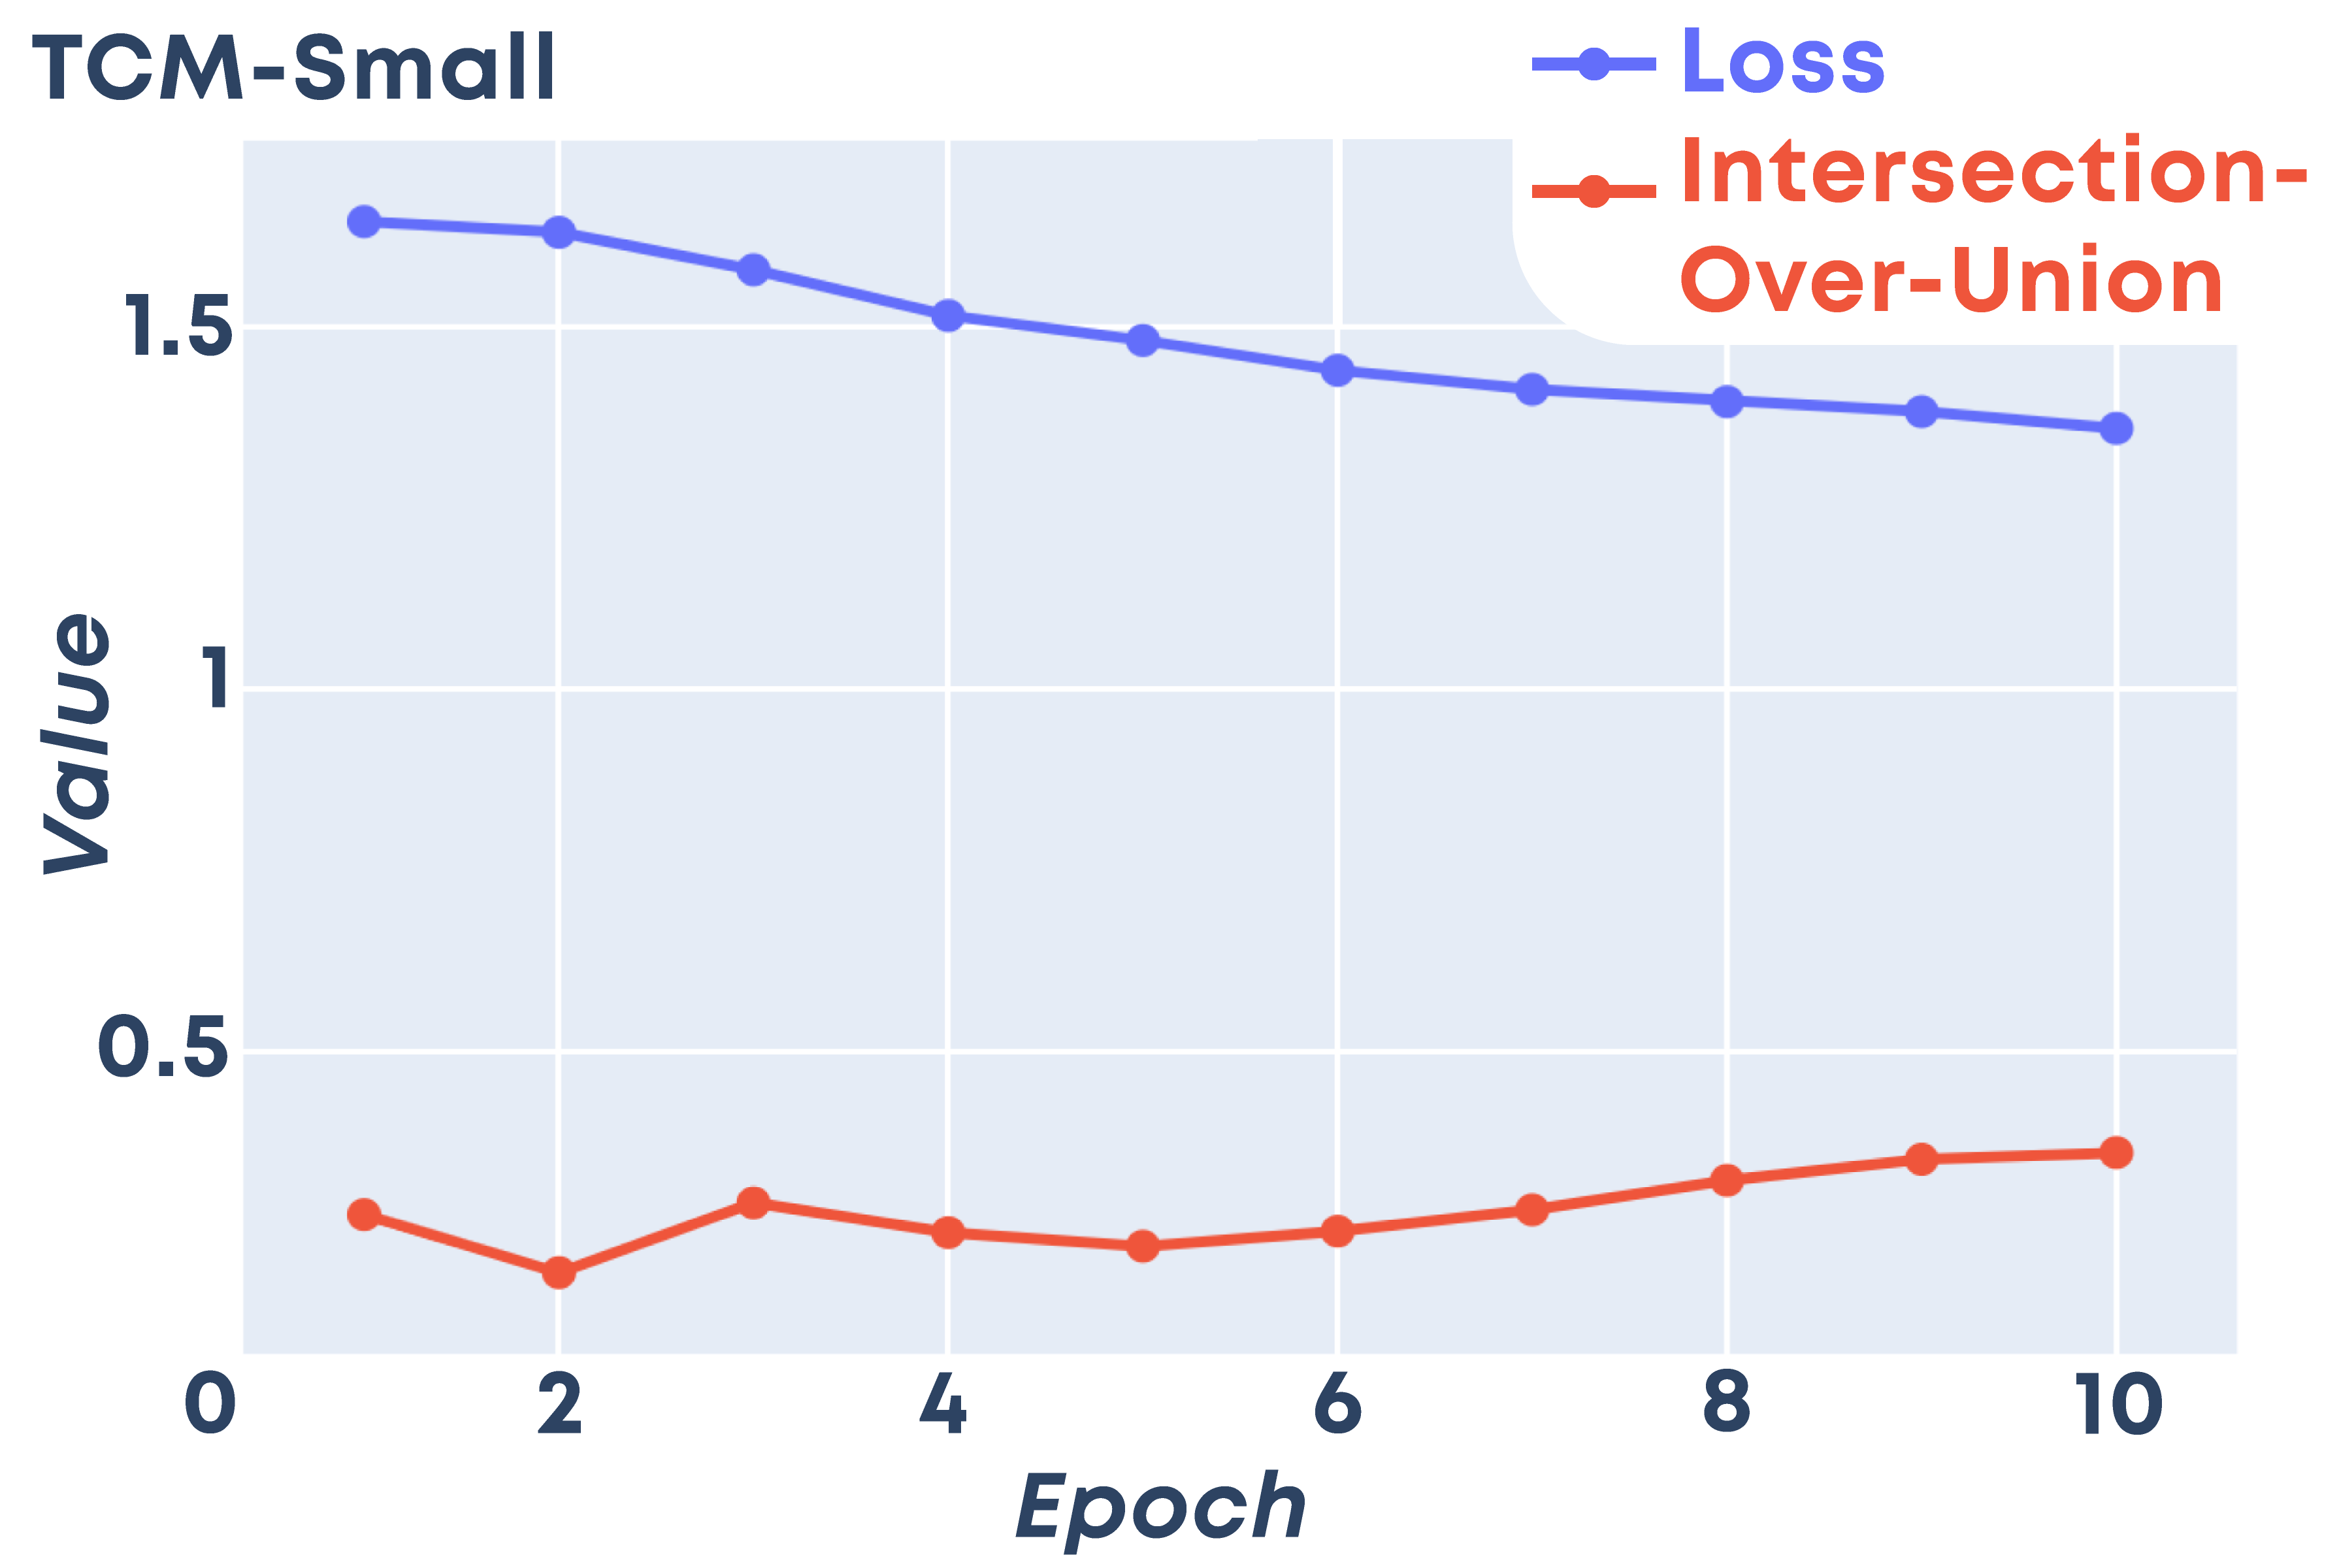
\includegraphics[width=1\linewidth]{fig6.png}
\caption{Training results of TCM-Small model.}
\label{fig}
\end{figure}

\begin{figure}[htbp]
\centering
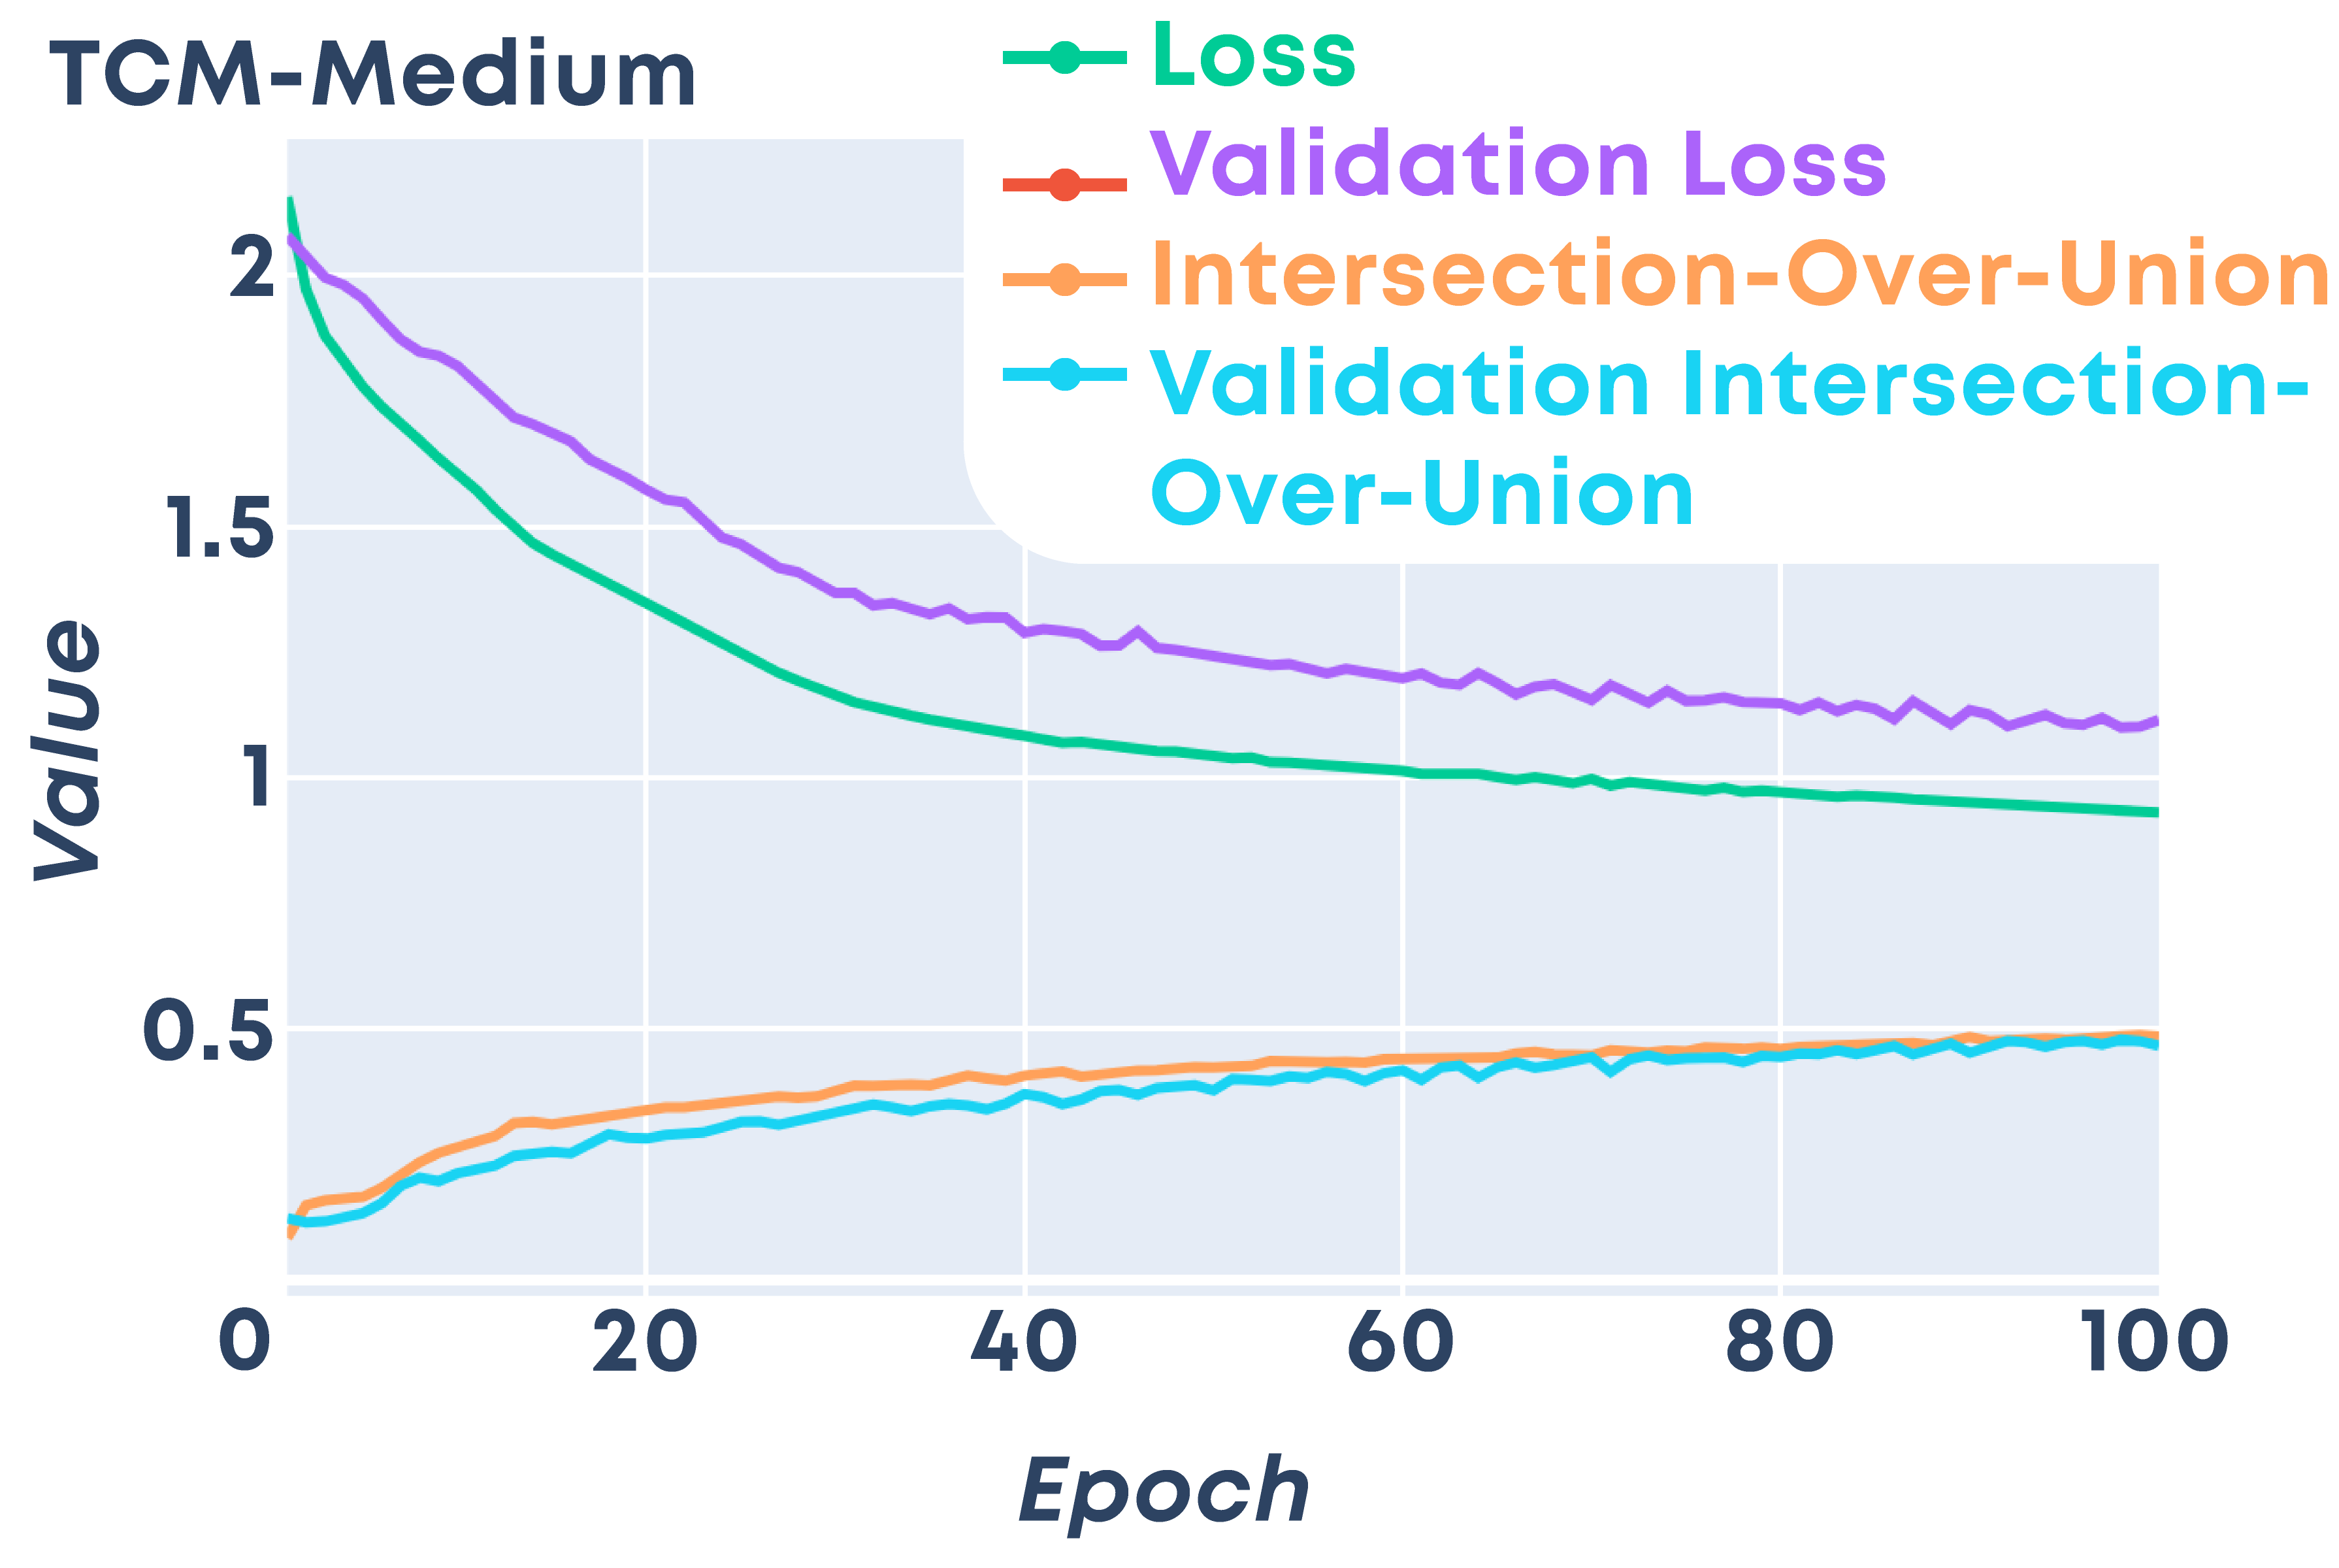
\includegraphics[width=1\linewidth]{fig7.png}
\caption{Training results of TCM-Medium model.}
\label{fig}
\end{figure}

In both Figures 6 and 7, the learning process was compared in terms of training loss and validation loss. Additionally, there was applied the Intersection-Over-Union test metric which allows us to see the overlay metric of segmentation masks. The larger this indicator, the better the process of overlaying and classification in the model. Thus, the trend is clear that models do not provide sharp progress and results in the learning process, even though the association between val and loss is basically valid. Although these observations suggest the absence of clear indications of overfitting or underfitting tendencies within the models, the training process lacks pronounced improvements. It points towards potential challenges in model performance and optimization. Further analysis and investigation are necessary to identify and address the factors contributing to this phenomenon.

From a practical standpoint, there is potential for the deployment of these models in a simple application via Hugging Faces or other services. For instance, one of the most popular third-party visual libraries in Python for building quick local and web apps for the MLOps (Machine Learning Operations) pipeline is Streamlit \cite{b12}. It contains pre-made visual components that can be put together as a constructor in it. The Figure 8 shows the interface of this application based on the TCM-Large model, in which there is a choice of location by name and coordinates, date frames, patch size, and image scale. Scale contributes to "compressing" the image so that it displays more or less meters per pixel. Its default is 10 meters per pixel. On the other hand, the patch size is potentially unlimited, but the Google Cloud API does not allow sending too much data and limits traffic for individual accounts. For this case, a value of 512 is optimal, while 800 is a probable limit per data request.

\begin{figure}[htbp]
\centering
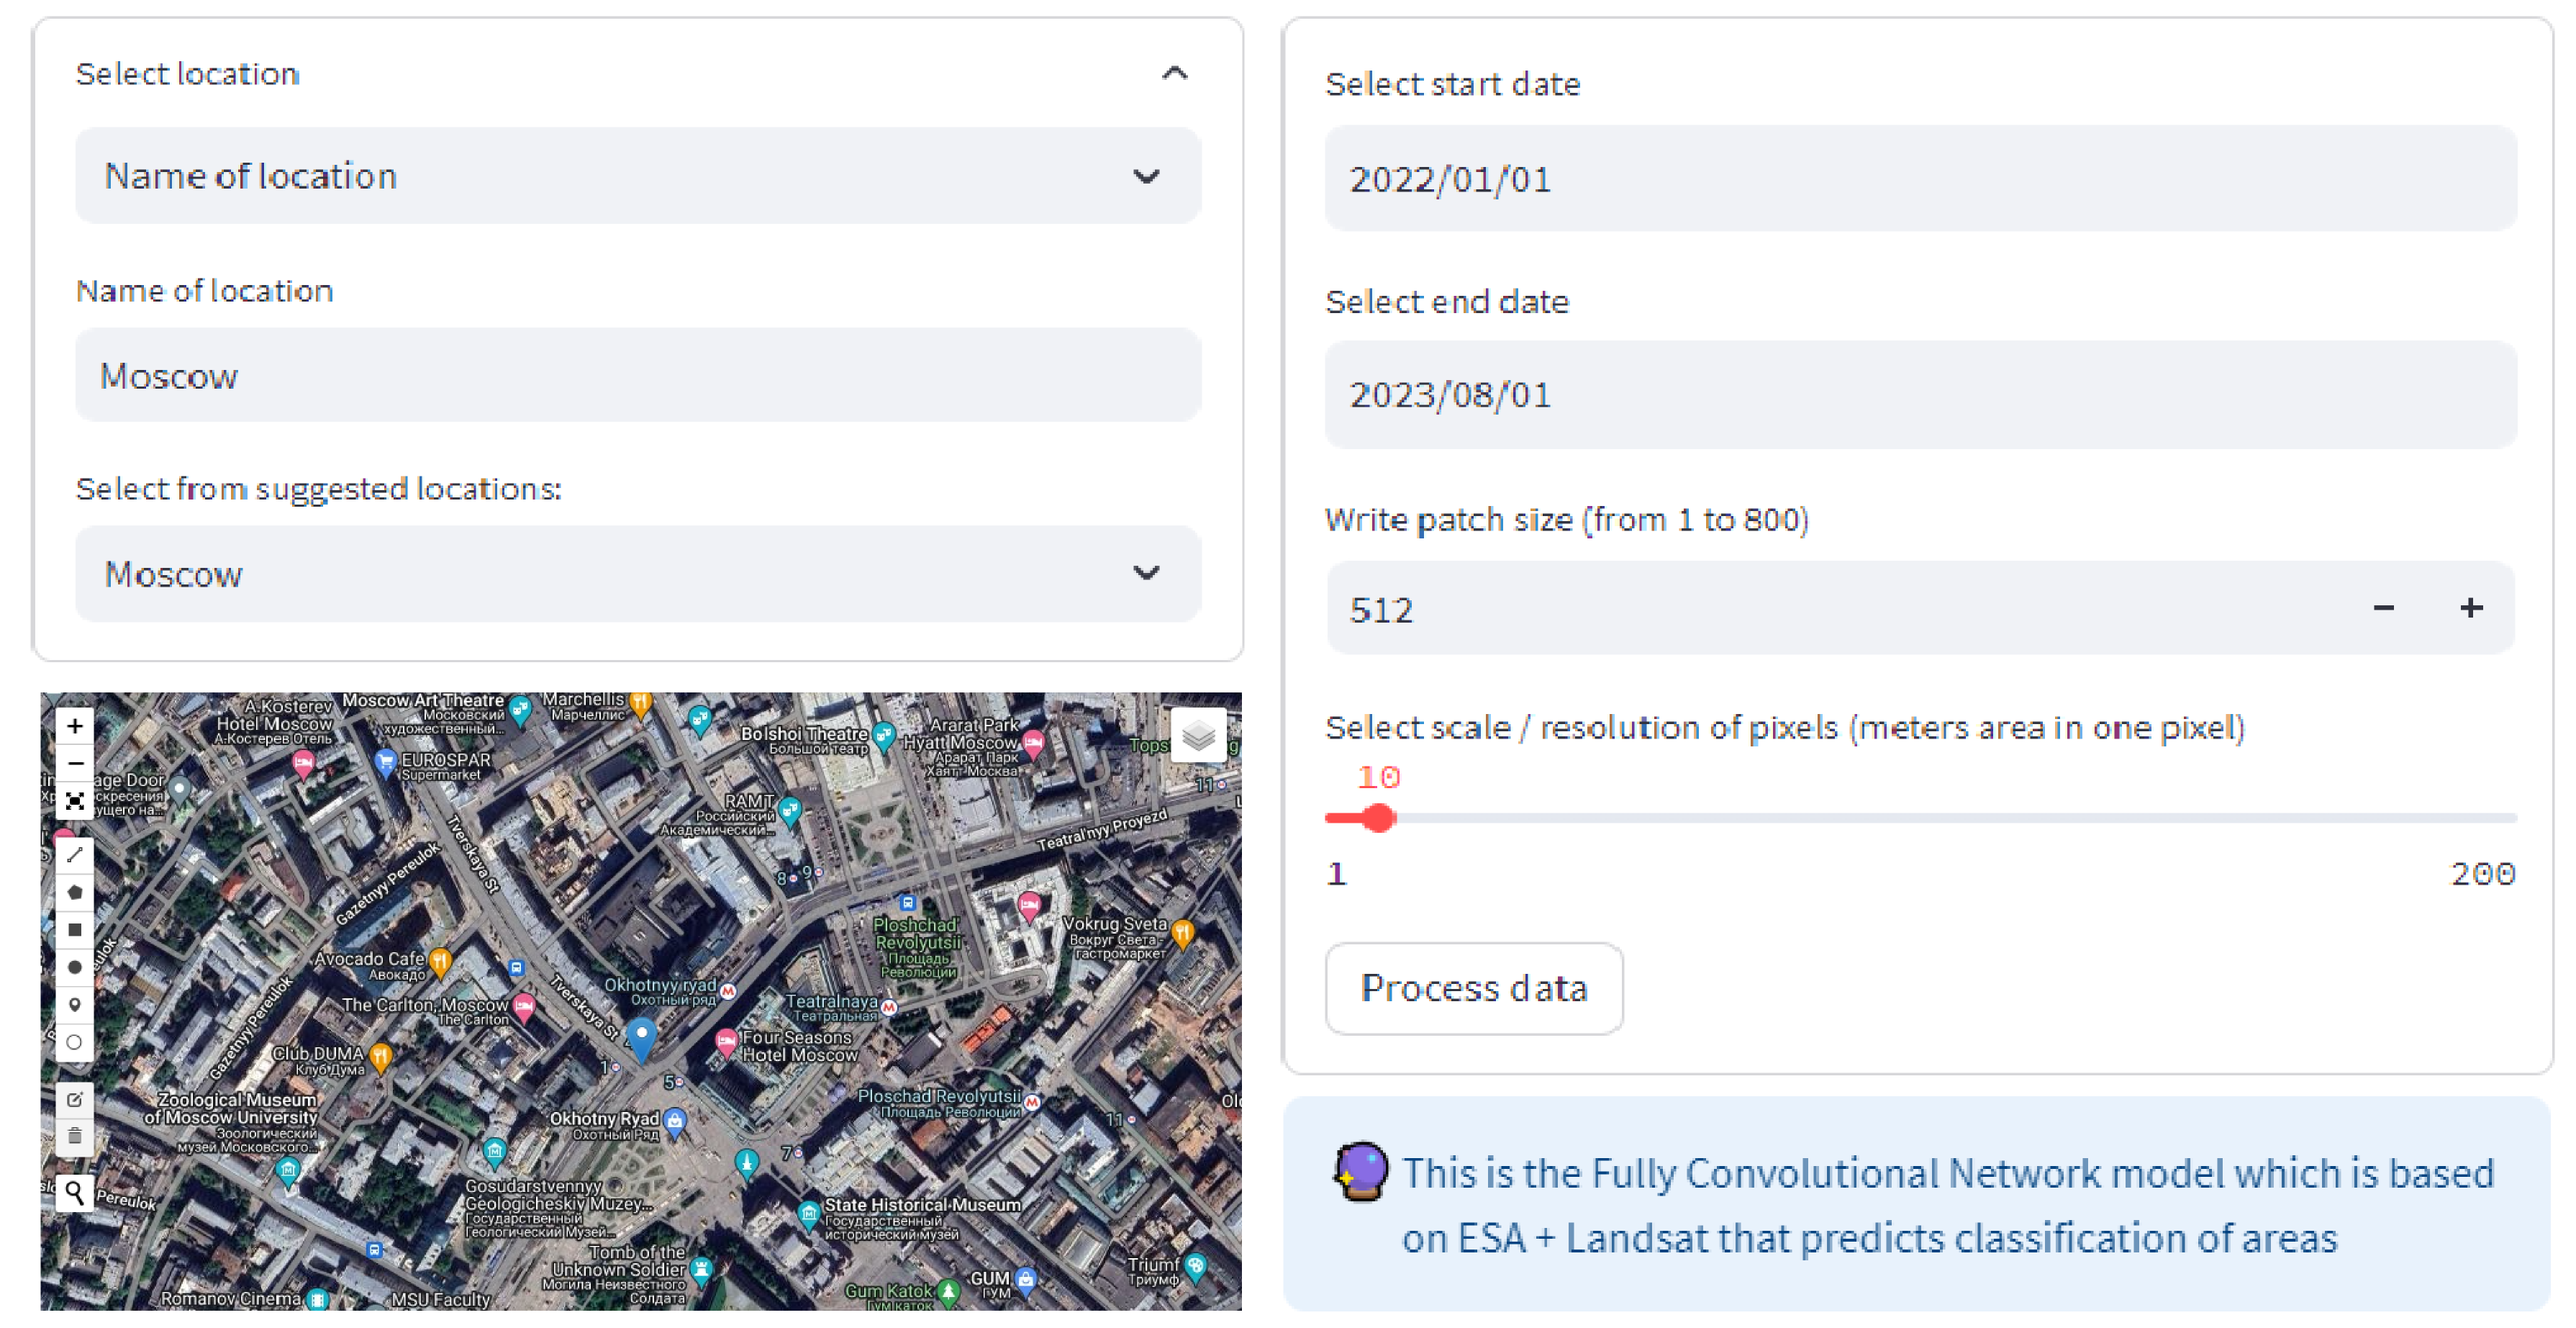
\includegraphics[width=0.95\linewidth]{fig8.png}
\caption{User Interface of TCM-Large App in Streamlit.}
\label{fig}
\end{figure}

Subsequently, another model test was conducted, but with a larger scale parameter of 100 units, a different location, and a distinct time period. This test yielded intriguing results and dependencies, as evident in the Figure 9.

\begin{figure}[htbp]
\centering
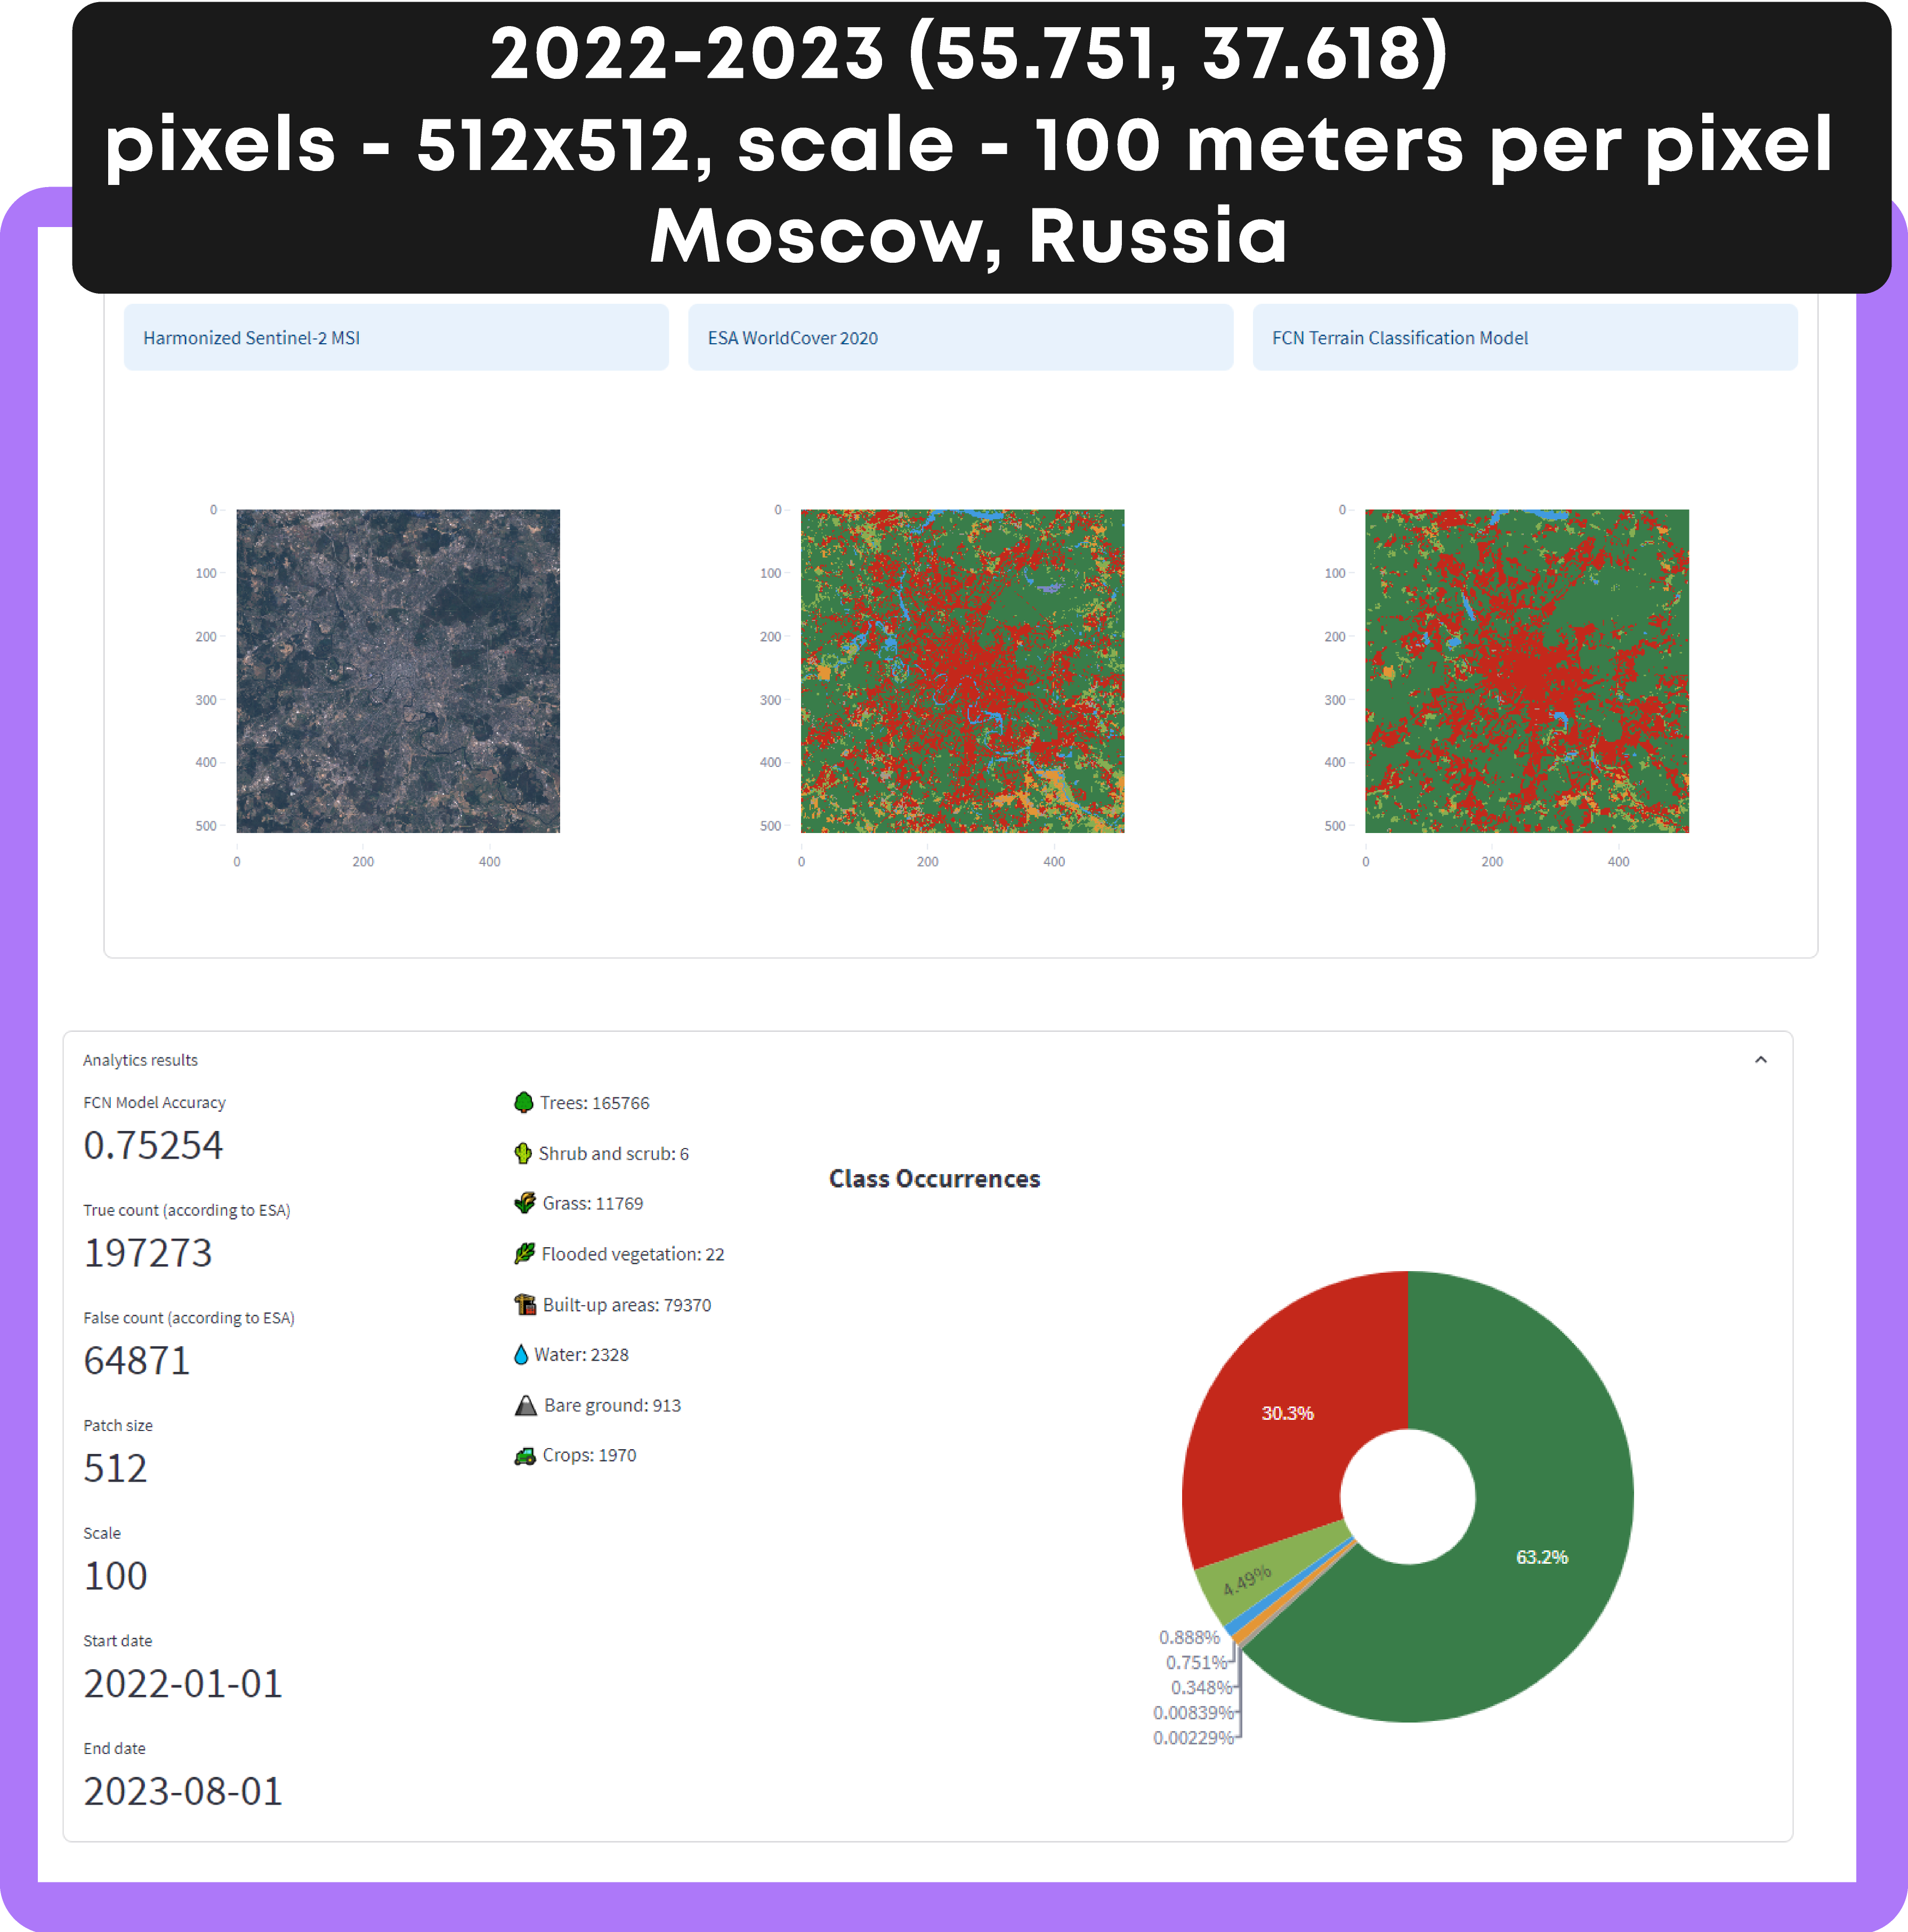
\includegraphics[width=1\linewidth]{fig9.png}
\caption{Results of TCM-Large with visual predictions comparison in Streamlit.}
\label{fig}
\end{figure}

Firstly, the model demonstrated competent classification of forested areas. Secondly, the model provided less noisy outcomes for larger territories, exhibiting more distinct and sizable clusters. Thirdly, however, because of that reduced noise, there is a loss of fine details. For example, the recognition of river channels and water hollows became less visible. As a result, indicators of accuracy exceed even up to 75\%, suggesting that the application might be suitable for simplified and rapid territorial analysis, as demonstrated in the Table 2.

\begin{table}[htbp]
\centering
\caption{Calculated processing time per product of TCM-Large model}
\label{tab}
\begin{tabular}{l|c|c|c|c}
\toprule
\textbf{Scale / Resolution} & \textbf{128px} & \textbf{256px} & \textbf{512px} & \textbf{800px}\\
\midrule
10 meters & 0.077s & 0.110s & 0.242s & 1.515s\\
20 meters & 0.085s & 0.231s & 0.287s & 1.618s\\
80 meters & 0.124s & 0.263s & 0.324s & 1.670s\\
\bottomrule
average & 0.095s & 0.201s & 0.284s & 1.601s\\
median & 0.085s & 0.231s & 0.287s & 1.618s\\
\bottomrule
\end{tabular}
\end{table}

When the scale parameter is modified, the processing speed of data per product is not significantly reduced. Between them, there is a variation of around 10\%. It is apparent that the model has more difficult classification processing when the resolution is increased from 500 to 800 pixels, which results in an increase of up to 1.5 seconds of return per product.

\section{Conclusion}

This research paper was aimed at trying to simplify the creation of terrain classification models based on FCNN and satellite information. By leveraging the power of data from ESA satellites, we have achieved minor-to-average results. It should be noted that the FCNN structure allows for working with images of various resolutions or scales, so it is not limited to certain options. However, it is required to combine the architecture of the model with alternative approaches such as U-Net or improve the learning process of the model. In general, the research project was focused on testing the relevance of the FCNN or CNN model structure in rapid GIS monitoring for potential application in real-life or practical services. For greater clarity, an application based on the Streamlit library was developed. It can be expanded and further integrated with other services or tools.

\section{Acknowledgments}

The article was written within the state order for the implementation of the scientific program under the budget program of the Republic of Kazakhstan 217 "Development of Science", subprogram 101 "Program-targeted funding of the scientific and/or technical activity at the expense of the national budget" on the theme: " Development of technology for intelligent preprocessing of aerospace images for recognition and identification of various objects " Grant IRN AP19678773.

\begin{thebibliography}{00}
\bibitem{b1} D. Kunertova, “The Ukraine Drone Effect on European Militaries,” Center for Security Studies, vol. 10 (15), no. 1, pp. 1-4, 2022, doi: 10.3929/ethz-b-000584078.
\bibitem{b2} Horning, N. Land cover classification methods. American Museum of Natural History, Center for Biodiversity and Conservation. 2004. [Online]. Available: http://biodiversityinformatics.amnh.org. Accessed: June. 27, 2023.
\bibitem{b3} F. Al-Ahmadi and A. Hames, “Comparison of Four Classification Methods to Extract Land Use and Land Cover from Raw Satellite Images for Some Remote Arid Areas, Kingdom of Saudi Arabia,” Journal of King Abdulaziz University-Earth Sciences, vol. 20, no. 1, pp. 167–191, 2009, doi: https://doi.org/10.4197/ear.20-1.9.
\bibitem{b4} Murali Krishna Gumma et al., “Agricultural cropland extent and areas of South Asia derived using Landsat satellite 30-m time-series big-data using random forest machine learning algorithms on the Google Earth Engine cloud,” vol. 57, no. 3, pp. 302–322, Nov. 2019, doi: https://doi.org/10.1080/15481603.2019.1690780.
\bibitem{b5} D. C. Duro, S. E. Franklin, and M. G. Dubé, “A comparison of pixel-based and object-based image analysis with selected machine learning algorithms for the classification of agricultural landscapes using SPOT-5 HRG imagery,” Remote Sensing of Environment, vol. 118, pp. 259–272, Mar. 2012, doi: https://doi.org/10.1016/j.rse.2011.11.020.
\bibitem{b6} S. Bhatnagar, L. Gill, and B. Ghosh, “Drone Image Segmentation Using Machine and Deep Learning for Mapping Raised Bog Vegetation Communities,” Remote Sensing, vol. 12, no. 16, p. 2602, Aug. 2020, doi: https://doi.org/10.3390/rs12162602.
\bibitem{b7} J. H. Jeppesen, R. H. Jacobsen, F. Inceoglu, and T. S. Toftegaard, “A cloud detection algorithm for satellite imagery based on deep learning,” Remote Sensing of Environment, vol. 229, pp. 247–259, Aug. 2019, doi: https://doi.org/10.1016/j.rse.2019.03.039.
\bibitem{b8} M. Zhang, H. Lin, G. Wang, H. Sun, and J. Fu, “Mapping Paddy Rice Using a Convolutional Neural Network (CNN) with Landsat 8 Datasets in the Dongting Lake Area, China,” Remote Sensing, vol. 10, no. 11, p. 1840, Nov. 2018, doi: https://doi.org/10.3390/rs10111840.
\bibitem{b9} M. K. Bennett, N. Younes, and K. Joyce, “Automating Drone Image Processing to Map Coral Reef Substrates Using Google Earth Engine,” Drones, vol. 4, no. 3, p. 50, Aug. 2020, doi: https://doi.org/10.3390/drones4030050.
\bibitem{b10} D. Phiri, M. Simwanda, S. Salekin, V. R. Nyirenda, Y. Murayama, and M. Ranagalage, “Sentinel-2 Data for Land Cover/Use Mapping: A Review,” Remote Sensing, vol. 12, no. 14, p. 2291, Jul. 2020, doi: https://doi.org/10.3390/rs12142291.
\bibitem{b11} G. Berg, “Image Classification with Machine Learning as a Service: - A comparison between Azure, SageMaker, and Vertex AI,” Dissertation, 2022.
\bibitem{b12} S. Wazir, G. S. Kashyap, and P. Saxena, “MLOps: A Review,” arXiv (Cornell University), Aug. 2023, doi: https://doi.org/10.48550/arxiv.2308.10908.
\end{thebibliography}

\end{document}